\documentclass[12pt, a4paper, onecolumn]{article} 
\usepackage{pdfpages}
\usepackage[utf8]{inputenc}
\usepackage{fancyhdr}
\usepackage{graphicx}
\usepackage{geometry}
\usepackage{float}
\usepackage{multicol} % Ajout du paquet multicol pour gérer les colonnes
\usepackage{lmodern}  % Latin Modern scalable font
\usepackage[T1]{fontenc}  % Use T1 font encoding
\usepackage{hyperref}  % Pour rendre la table des matières interactive




% Réduire les marges
\geometry{top=1.5cm, bottom=1.5cm, left=1.5cm, right=1.5cm}

%%%%%%%%%%%%%%%%%%%%%%%%%%%%%%%%%%%%%%%%%
% Wenneker Article
% Structure Specification File
% Version 1.0 (28/2/17)
%
% This file originates from:
% http://www.LaTeXTemplates.com
%
% Authors:
% Frits Wenneker
% Vel (vel@LaTeXTemplates.com)
%
% License:
% CC BY-NC-SA 3.0 (http://creativecommons.org/licenses/by-nc-sa/3.0/)
%
%%%%%%%%%%%%%%%%%%%%%%%%%%%%%%%%%%%%%%%%%

%----------------------------------------------------------------------------------------
%	PACKAGES AND OTHER DOCUMENT CONFIGURATIONS
%----------------------------------------------------------------------------------------

\usepackage[english]{babel} % English language hyphenation

\usepackage{microtype} % Better typography

\usepackage{amsmath,amsfonts,amsthm} % Math packages for equations

\usepackage[svgnames]{xcolor} % Enabling colors by their 'svgnames'

\usepackage[hang, small, labelfont=bf, up, textfont=it]{caption} % Custom captions under/above tables and figures

\usepackage{booktabs} % Horizontal rules in tables

\usepackage{lastpage} % Used to determine the number of pages in the document (for "Page X of Total")

\usepackage{graphicx} % Required for adding images

\usepackage{enumitem} % Required for customising lists
\setlist{noitemsep} % Remove spacing between bullet/numbered list elements

\usepackage{sectsty} % Enables custom section titles
\allsectionsfont{\usefont{OT1}{phv}{b}{n}} % Change the font of all section commands (Helvetica)

%----------------------------------------------------------------------------------------
%	MARGINS AND SPACING
%----------------------------------------------------------------------------------------

\usepackage{geometry} % Required for adjusting page dimensions

\geometry{
	top=1cm, % Top margin
	bottom=1.5cm, % Bottom margin
	left=2cm, % Left margin
	right=2cm, % Right margin
	includehead, % Include space for a header
	includefoot, % Include space for a footer
	%showframe, % Uncomment to show how the type block is set on the page
}

\setlength{\columnsep}{7mm} % Column separation width

%----------------------------------------------------------------------------------------
%	FONTS
%----------------------------------------------------------------------------------------

\usepackage[T1]{fontenc} % Output font encoding for international characters
\usepackage[utf8]{inputenc} % Required for inputting international characters

\usepackage{XCharter} % Use the XCharter font

%----------------------------------------------------------------------------------------
%	HEADERS AND FOOTERS
%----------------------------------------------------------------------------------------

\usepackage{fancyhdr} % Needed to define custom headers/footers
\pagestyle{fancy} % Enables the custom headers/footers

\renewcommand{\headrulewidth}{0.0pt} % No header rule
\renewcommand{\footrulewidth}{0.4pt} % Thin footer rule

\renewcommand{\sectionmark}[1]{\markboth{#1}{}} % Removes the section number from the header when \leftmark is used

%\nouppercase\leftmark % Add this to one of the lines below if you want a section title in the header/footer

% Headers
\lhead{} % Left header
\chead{\textit{\thetitle}} % Center header - currently printing the article title
\rhead{} % Right header

% Footers
\lfoot{} % Left footer
\cfoot{} % Center footer
\rfoot{\footnotesize Page \thepage\ of \pageref{LastPage}} % Right footer, "Page 1 of 2"

\fancypagestyle{firstpage}{ % Page style for the first page with the title
	\fancyhf{}
	\renewcommand{\footrulewidth}{0pt} % Suppress footer rule
}

%----------------------------------------------------------------------------------------
%	TITLE SECTION
%----------------------------------------------------------------------------------------

\newcommand{\authorstyle}[1]{{\large\usefont{OT1}{phv}{b}{n}\color{Red}#1}} % Authors style (Helvetica)

\newcommand{\institution}[1]{{\footnotesize\usefont{OT1}{phv}{m}{sl}\color{Black}#1}} % Institutions style (Helvetica)

\usepackage{titling} % Allows custom title configuration

\newcommand{\HorRule}{\color{White}\rule{\textwidth}{5pt}} 
\newcommand{\mydate}{\hfill \textbf{\today}} % Met en gras et aligne à gauche


\pretitle{
	\vspace{-30pt} % Move the entire title section up
	\HorRule\vspace{10pt} % Horizontal rule before the title
	\fontsize{32}{36}\usefont{OT1}{phv}{b}{n}\selectfont % Helvetica
	\color{Red} % Text colour for the title and author(s)
}

\posttitle{\par\vskip 15pt} % Whitespace under the title

\preauthor{} % Anything that will appear before \author is printed

\postauthor{ % Anything that will appear after \author is printed
	\vspace{10pt} % Space before the rule
	\par\HorRule % Horizontal rule after the title
	\vspace{20pt} % Space after the title section
}

%----------------------------------------------------------------------------------------
%	ABSTRACT
%----------------------------------------------------------------------------------------

\usepackage{lettrine} % Package to accentuate the first letter of the text (lettrine)
\usepackage{fix-cm}	% Fixes the height of the lettrine

\newcommand{\initial}[1]{ % Defines the command and style for the lettrine
	\lettrine[lines=3,findent=4pt,nindent=0pt]{% Lettrine takes up 3 lines, the text to the right of it is indented 4pt and further indenting of lines 2+ is stopped
		\color{DarkGoldenrod}% Lettrine colour
		{#1}% The letter
	}{}%
}

\usepackage{xstring} % Required for string manipulation

\newcommand{\lettrineabstract}[1]{
	\StrLeft{#1}{1}[\firstletter] % Capture the first letter of the abstract for the lettrine
	\initial{\firstletter}\textbf{\StrGobbleLeft{#1}{1}} % Print the abstract with the first letter as a lettrine and the rest in bold
}

%----------------------------------------------------------------------------------------
%	BIBLIOGRAPHY
%----------------------------------------------------------------------------------------

\usepackage[backend=bibtex,style=authoryear,natbib=true]{biblatex} % Use the bibtex backend with the authoryear citation style (which resembles APA)

\addbibresource{example.bib} % The filename of the bibliography

\usepackage[autostyle=true]{csquotes} % Required to generate language-dependent quotes in the bibliography
 

%----------------------------------------------------------------------------------------
%	ARTICLE INFORMATION
%----------------------------------------------------------------------------------------

\title{Labo5 - POO \\ Matrices} 

% Modifiez le style des auteurs
\newcommand{\largename}[1]{{\Large\textbf{#1}}} % style pour le nom de famille

\author{
	\authorstyle{Dani Tiago \largename{Faria dos Santos}\\ Antoine \largename{Aubry } \\ \\ Groupe  \textbf{L02GrD}\\ HEIG-VD} % Authors
}

\makeatletter
\renewcommand\date[1]{\gdef\@date{\hbox to \linewidth{#1\hss}}}
\makeatother
\date{\today}


\pagestyle{fancy}
\fancyhf{}
\fancyhead[L]{Laboratoire 5 - POO}
\fancyhead[R]{Groupe L03GrD}
\fancyfoot[R]{Page \thepage}
\fancyfoot[L]{HEIG-VD | Dani Tiago \textbf{Faria dos Santos} - Antoine \textbf{Aubry }}


% Ligne sous l'en-tête
\renewcommand{\headrulewidth}{0.7pt}
% Pas de ligne sur le pied de page
\renewcommand{\footrulewidth}{0.5pt}


\begin{document}
	% Utilisation de twocolumn pour le titre
	\twocolumn[ 
	\maketitle
	]
	
	% Retour à une seule colonne
	\onecolumn 
	
	% Table des matières
	\tableofcontents
	\newpage
	
	\section{Modélisation UML}
	\begin{figure}[H]
	\centering
	\includegraphics[width=1\textwidth]{../schema.png}
	\caption{Implémentation de la modélisation de la classe Matrix}
\end{figure}
	
	\section{Choix de Conception}
	\begin{flushleft}
\begin{enumerate}
	\item \textbf{Encapsulation} : 
	La classe \texttt{Matrix} protège ses attributs (dimensions, éléments, modulo) à l'aide de modificateurs d'accès, garantissant ainsi l'intégrité des données et minimisant les accès non autorisés.
	
	\item \textbf{Gestion des Exceptions} : 
	Des exceptions (\texttt{RuntimeException}) sont lancées pour gérer les cas de paramètres non valides, comme des dimensions négatives ou des modulos différents, permettant ainsi une gestion robuste des erreurs.
	
	\item \textbf{Modélisation Orientée Objet} : 
	Les opérations arithmétiques (addition, soustraction, multiplication) sont modélisées via des classes spécifiques (par exemple, \texttt{Addition}, \texttt{Subtraction}, \texttt{Multiplication}). Cela permet une factorisation du code et une extensibilité, facilitant l'ajout de nouvelles opérations à l'avenir.
	
	\item \textbf{Gestion des Dimensions} : 
	Lors de l'opération entre matrices de tailles différentes, le résultat est une nouvelle matrice de taille maximale avec des valeurs manquantes remplacées par des zéros, ce qui assure une manipulation cohérente des données.

    \item \textbf{Centralisation du Code Commun} : 
	Le code commun aux différentes opérations est encapsulé pour éviter la duplication, ce qui permet d'ajouter facilement de nouvelles opérations sans nécessiter de structures de contrôle complexes comme \texttt{if} ou \texttt{switch}.

\end{enumerate}
\end{flushleft}
	
	\section{Listing du Code des Tests}
	\subsection{Test de la classe Matrix}

	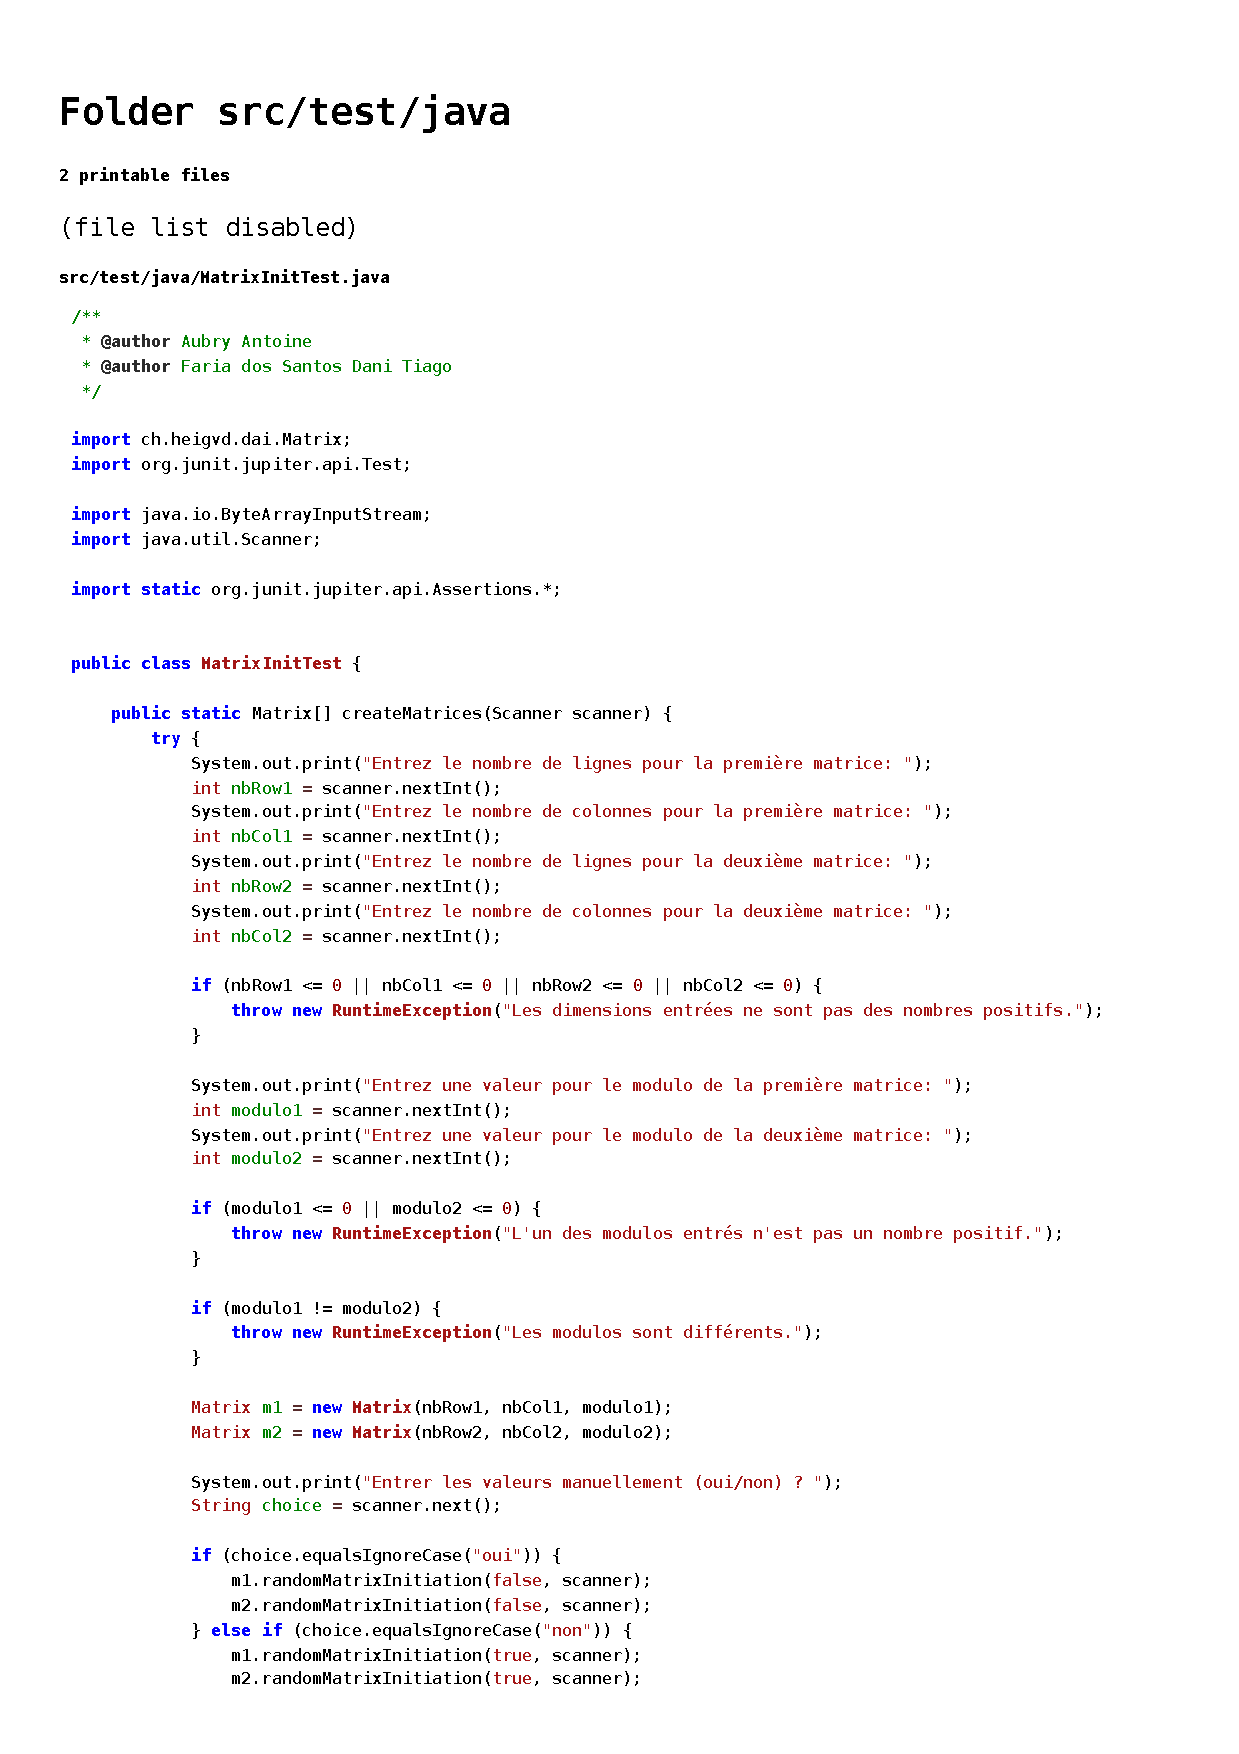
\includepdf[pages=-]{src_test_java.pdf}
	

	\newpage
	
	\section{Documentation des Tests Effectués}
	\subsection{Tests de la Classe \texttt{Matrix}}
	
	\begin{itemize}
		\item \textbf{testAdditionOperation()}
		\begin{itemize}
			\item \textbf{Description} : Teste l'addition de deux matrices.
			\item \textbf{Entrées} : \texttt{matrix1} contenant les valeurs $\begin{bmatrix} 1 & 2 \\ 3 & 4 \end{bmatrix}$ et \texttt{matrix2} contenant $\begin{bmatrix} 5 & 6 \\ 7 & 8 \end{bmatrix}$.
			\item \textbf{Résultats Attendus} : Les éléments résultants doivent être $\begin{bmatrix} 6 & 8 \\ 10 & 12 \end{bmatrix}$.
		\end{itemize}
		
		\item \textbf{testSubtractionOperation()}
		\begin{itemize}
			\item \textbf{Description} : Teste la soustraction de deux matrices.
			\item \textbf{Entrées} : \texttt{matrix1} et \texttt{matrix2} comme ci-dessus.
			\item \textbf{Résultats Attendus} : Les éléments résultants doivent être $\begin{bmatrix} -4 & -4 \\ -4 & -4 \end{bmatrix}$.
		\end{itemize}
		
		\item \textbf{testMultiplicationOperation()}
		\begin{itemize}
			\item \textbf{Description} : Teste la multiplication de deux matrices.
			\item \textbf{Entrées} : \texttt{matrix1} et \texttt{matrix2} comme ci-dessus.
			\item \textbf{Résultats Attendus} : Les éléments résultants doivent être $\begin{bmatrix} 19 & 22 \\ 43 & 50 \end{bmatrix}$.
		\end{itemize}
		
		\item \textbf{testMatrixInitialization()}
		\begin{itemize}
			\item \textbf{Description} : Vérifie que les matrices sont correctement initialisées.
			\item \textbf{Résultats Attendus} : Les matrices ne doivent pas être nulles après initialisation.
		\end{itemize}
		
		\item \textbf{testValueSettingAndGetting()}
		\begin{itemize}
			\item \textbf{Description} : Vérifie la possibilité de définir et d'obtenir des valeurs dans la matrice.
			\item \textbf{Entrées} : Valeurs initiales et modifications.
			\item \textbf{Résultats Attendus} : Les valeurs doivent être correctement mises à jour et récupérées.
		\end{itemize}
		
		\item \textbf{testDisplay()}
		\begin{itemize}
			\item \textbf{Description} : Teste que la méthode d'affichage ne lève pas d'exceptions.
			\item \textbf{Résultats Attendus} : L'appel de la méthode d'affichage ne doit pas provoquer d'erreur.
		\end{itemize}
	\end{itemize}
		\newpage
	\subsection{Tests d'Initialisation des Matrices}
	
	\begin{itemize}
		\item \textbf{testCreateMatricesWithValidInput()}
		\begin{itemize}
			\item \textbf{Description} : Teste la création de matrices avec des entrées utilisateur valides.
			\item \textbf{Entrées} : Dimensions et valeurs définies par l'utilisateur.
			\item \textbf{Résultats Attendus} : Les matrices doivent être créées avec les dimensions et valeurs correctes.
		\end{itemize}
		
		\item \textbf{testCreateMatricesWithInvalidDimensions()}
		\begin{itemize}
			\item \textbf{Description} : Vérifie que le système gère les dimensions invalides.
			\item \textbf{Entrées} : Dimensions négatives.
			\item \textbf{Résultats Attendus} : Une exception doit être levée avec un message approprié.
		\end{itemize}
		
		\item \textbf{testCreateMatricesWithDifferentModulos()}
		\begin{itemize}
			\item \textbf{Description} : Teste la création de matrices avec des modulos différents.
			\item \textbf{Entrées} : Modulos non identiques.
			\item \textbf{Résultats Attendus} : Une exception doit être levée avec un message indiquant que les modulos sont différents.
		\end{itemize}
	\end{itemize}
	
	
	
	
\end{document}
